\appendix
\section{BAMCP} \label{bamcp}

\begin{algorithm}[h]
  \caption{BAMCP}
  \label{alg:1}
  \begin{multicols}{2}
    \begin{algorithmic}
      \State
      \State \textbf{Input:} $\pi$, $E$, $d_{\text{max}}$, $\mathcal{R}$, $\gamma$, $\mathcal{A}$, $c$
      \State
      \Procedure{Search}{$(s, h), b(\theta)$}
        \For{$e=1 \cdots E$}
        \State $\theta \sim b(\cdot)$
        \State \textproc{Simulate}($(s, h), \theta, d_{\text{max}}$)
        \EndFor
        \State \Return $\arg \max_{a} Q((s, h), a)$
      \EndProcedure
      \State
      \Procedure{Rollout}{$(s, h), \theta, d$}
        \If{$d==0$}
        \State \Return 0
        \EndIf
        \State $a \sim \pi(\cdot|(s, h))$
        \State $s' \sim \mathcal{P}_\theta(\cdot|s, a)$
        \State $r \leftarrow \mathcal{R}(s, a)$
        \State {\small $R \leftarrow r + \gamma\textproc{Rollout}((s', has'), \theta, d - 1)$}
        \State \Return $R$
      \EndProcedure
    \end{algorithmic}
    \columnbreak
    \begin{algorithmic}
      \Procedure{Simulate}{$(s, h), \theta, d$}
        \If{$d==0$}
        \State \Return 0
        \EndIf
        \If{$N((s, h))==0$}
        \For{$a \in \mathcal{A}$}
        \State $N((s, h), a), Q((s, h), a) \leftarrow 0, 0$
        \EndFor
        \State $a \sim \pi(\cdot|(s, h))$
        \State $s' \sim \mathcal{P}_\theta(\cdot|s, a), r \leftarrow \mathcal{R}(s, a)$
        \State {\small $R \leftarrow r + \gamma \textproc{Rollout}((s', has'), \theta, d - 1)$}
        \State $N((s, h)), N((s, h), a) \leftarrow 1, 1$
        \State $Q((s, h), a) \leftarrow R$
        \State \Return $R$
        \EndIf
        \State {\small $a \leftarrow \arg \max_{x} Q((s, h), x) + c \sqrt{\frac{\log N((s, h))}{N((s, h), x)}}$} 
        \State $s' \sim \mathcal{P}_\theta(\cdot|s, a), r \leftarrow \mathcal{R}(s, a)$
        \State {\small $R \leftarrow r + \gamma \textproc{Simulate}((s', has'), \theta, d - 1)$}
        \State $N((s, h)) \mathrel{{+}{=}} 1, N((s, h), a) \mathrel{{+}{=}} 1$
        \State $Q((s, h), a) \mathrel{{+}{=}} \frac{R - Q((s, h), a)}{N((s, h), a)}$
        \State \Return $R$ 
      \EndProcedure
    \end{algorithmic}
  \end{multicols}
\end{algorithm}

Bayes Adaptive Monte Carlo Planning (BAMCP, \cite{DBLP:journals/jair/GuezSD13}) is a sample-based online planning method, aiming to find the action $a^*$ that approximately maximizes the expected return at a decision point $(s, h)$ under the BAMDP. Its detailed pseudo code is shown as Algorithm \ref{alg:1}. BAMCP has demonstrated success in solving BAMDPs with large-scale \textbf{discrete} state and action spaces. Its key algorithmic ideas include: (1) applying MCTS with an efficient exploration strategy -- UCT (\cite{DBLP:conf/ecml/KocsisS06}) to the BAMDP in order to simulate the outcomes of different action choices; (2) utilizing root sampling to avoid frequent Bayesian posterior updates. Specifically, the UCT rule is used for selecting actions at non-leaf nodes, i.e., {\small $a \leftarrow \arg \max_{x} Q((s, h), x) + c \sqrt{\frac{\log N((s, h))}{N((s, h), x)}}$}, managing the tradeoff between exploration and exploitation. Root sampling refers to sampling the dynamics model only at the root node (i.e., $\theta \sim b(\cdot)$) and not adapting the belief $b(\cdot)$ according to the Bayes rule during the search process, of which the rationality is justified in the following lemma.
\begin{lemma} \label{lem:1}
For all suffix histories $h'$ of $h$, $b(\theta|h') = \Tilde{b}(\theta|h')$. Here, $b(\theta|h')$ is the true posterior probability of $\theta$ at the decision point $h'$, while $\Tilde{b}(\theta|h')$ is the probability of experiencing $\theta$ at $h'$ when using root sampling.
\end{lemma}
\begin{proof}
This lemma can be proved by induction.

Base case: When $h'=h$, $b(\theta|h') = \Tilde{b}(\theta|h') = b(\theta)$.

Step case: 
\begin{equation} \label{root_sampling}
    \begin{aligned}
        b(\theta|has') & = P(has'|\theta) P(\theta) / P(has') \\
        & = P(h|\theta) \mathcal{P}_\theta(s'|s, a) P(\theta) / P(has') \\
        & = b(\theta|h)P(h) \mathcal{P}_\theta(s'|s, a) / P(has') \\
        & = Z b(\theta|h)\mathcal{P}_\theta(s'|s, a) \\
        & = Z \Tilde{b}(\theta|h) \mathcal{P}_\theta(s'|s, a) \\
        & = Z \Tilde{b}(\theta|ha) \mathcal{P}_\theta(s'|s, a) = \Tilde{b}(\theta|has')
    \end{aligned}
\end{equation}
Here, $Z = 1/\int_\theta \mathcal{P}_\theta(s'|s, a) b(\theta|h) d\theta = 1/\int_\theta \mathcal{P}_\theta(s'|s, a) \tilde{b}(\theta|h) d\theta = 1/\int_\theta \mathcal{P}_\theta(s'|s, a) \tilde{b}(\theta|ha) d\theta$ is the normalization constant. The fifth equality in Eq. (\ref{root_sampling}) holds due to the inductive hypothesis. The sixth equality is based on the fact that the choice of $a$ at each node $h$ is made independently of the sample $\theta$. As for the last equality, to experience $\theta$ at $has'$, the sample $\theta$ needs to traverse $ha$ (with probability $\tilde{b}(\theta|ha)$) and then the state $s'$ needs to be sampled, which is with probability $\mathcal{P}_\theta(s'|s, a)$, so $\Tilde{b}(\theta|has') \propto \tilde{b}(\theta|ha) \mathcal{P}_\theta(s'|s, a)$.
\end{proof}

\section{Alternative Design Choices for Continuous BAMCP} \label{alg1_details}

The terms labeled in blue in Algorithm \ref{alg:2} have alternative design choices. Empirical comparisons among these alternatives are reserved for future work.

$\tilde{Q}((s, h), x)$ in the exploration strategy, i.e., $a \leftarrow \arg \max_{x \in C((s, h))} \tilde{Q}((s, h), x)$, could take various forms. For instance, in (\cite{DBLP:conf/lion/CouetouxHSTB11, DBLP:journals/jair/GuezSD13, DBLP:conf/aaai/LeeJKK20}), $\tilde{Q}((s, h), x) = Q((s, h), x) + c \sqrt{\frac{\log N((s, h))}{N((s, h), x)}}$; in PUCT (\cite{DBLP:conf/pkdd/AugerCT13}), $\tilde{Q}((s, h), x) = Q((s, h), x) + \sqrt{\frac{N((s, h))^{e(d)}}{N((s, h), x)}}$, where $e(d)$ is a schedule of coefficients related to the search depth $d$; in Sampled MuZero (a variant of MuZero that can be applied in continuous action spaces (\cite{DBLP:conf/icml/HubertSABSS21})), $\tilde{Q}((s, h), x) = Q((s, h), x) + \hat{\pi}(x|(s, h)) \frac{\sqrt{N((s, h))}}{1+N((s, h), x)} \left(c_1 + \log \left(\frac{N((s,h))+c_2+1}{c_2}\right)\right)$.
% , which involves the being-learned policy $\pi$. 
Here, $c$, $c_1$, $c_2$ are hyperparameters, $\hat{\pi} = \hat{\beta} \pi^{1 - 1/\tau}$ is a sample policy defined upon the real policy $\pi$. In particular, at each decision point $(s, h)$, Sampled MuZero would sample $M$ actions $\{a_i\}$ from the distribution $\pi^{1/\tau}$ and accordingly define $\hat{\beta}(a|(s, h)) = \sum_{i} \mathds{1}_{a_i = a} / M$, where $\tau > 0$ is a temperature hyperparameter. Thus, Sampled MuZero does not adopt progressive widening like ours. Following BAMCP, we adopt the first definition of $\tilde{Q}((s, h), x)$, though it could potentially be improved with other choices. In addition, as an implementation trick (\cite{DBLP:conf/iclr/HamrickFBGVWABV21}), the Q estimates are usually normalized into $\bar{Q} \in [0, 1]$ before being used to calculate $\tilde{Q}$ as above. The normalized estimates can be computed as $\bar{Q}((s, h), x) = \frac{Q((s, h), x) - Q_{\text{min}}}{Q_{\text{max}} - Q_{\text{min}}}$, where $Q_{\text{max}}$ and $Q_{\text{min}}$ are the maximum and minimum Q values observed in the search tree so far.
% Moreover, to encourage additional exploration at the root node, a small amount of Dirichlet noise can be added to the policy $\pi$ at the root node alone.

As the planning/search result, $\pi_{\text{ret}}$ can take multiple forms. In (\cite{DBLP:journals/jair/GuezSD13, DBLP:conf/aips/SunbergK18, DBLP:conf/aaai/LeeJKK20}), $\pi_{\text{ret}}((s, h)) = \arg \max_{a \in C((s, h))} Q((s, h), a)$; in (Sampled) MuZero, $\pi_{\text{ret}}(a|(s, h)) = \frac{N((s, h), a)^{1/\tau}}{\sum_{x \in C((s, h))}N((s, h), x)^{1/\tau}}$; in ROSMO (a variant of MuZero with improved performance in offline scenarios (\cite{DBLP:conf/iclr/LiuLLYX23})), $\pi_{\text{ret}}(a|(s, h)) \propto \pi(a|(s, h)) \exp(Q((s, h), a) - V((s, h)))$. Here, $\tau \in (0, 1]$ is a temperature parameter and decays with the training process, ensuring the action selection becomes greedier. We select the second form for $\pi_{\text{ret}}$ in Algorithm \ref{alg:2}. This is because (1) as described in PUCT, the returned action should be the most visited one, which is not necessarily the one with the highest Q value, and (2) ROSMO adopts one-step look-ahead rather than deep tree search at each root node, which does not align with our approach.

As for the conditions of double progressive widening, PUCT designs $\alpha$ and $\beta$ to be functions of the search depth $d$, while UCT-DPW (\cite{DBLP:conf/lion/CouetouxHSTB11}) utilizes a different set of conditions: $\left \lceil {K_a N((s, h))^\alpha}\right \rceil \geq |C((s, h))|$, $\left \lceil {K_s N((s, h), a)^\beta}\right \rceil \geq |C((s, h), a)|$, where $K_a, K_s, \alpha, \beta$ are all constant hyperparameters. When the progressive widening condition for sampling the next state is not satisfied, either the least visited node in \(C((s, h), a)\) can be selected (following PUCT), or a random node can be sampled from \(C((s, h), a)\) following a distribution proportional to the number of visits (following UCT-DPW). As shown in Algorithm \ref{alg:2}, we follow the designs of PUCT, but keep $\alpha$ and $\beta$ as constants for simplicity in hyperparameter fine-tuning. 

Finally, the condition for continuing the simulation procedure, i.e., $N((s, h)) > 1$, could potentially be replaced with $N((s, h), a) > 1$ or $N((s', hars')) > 0$. These conditions indicate that the nodes $(s, h)$, $(s, h, a)$, and $(s', hars')$ have been visited before, respectively. At the end of the simulation procedure, we can either apply rollouts, i.e., simulating a single path until the end of an episode, to estimate the expected value for a leaf node \((s, h)\), or directly use \(V((s, h))\) as the estimation. The former approach is widely used in online planning algorithms (\cite{DBLP:journals/jair/GuezSD13, DBLP:conf/aips/SunbergK18, DBLP:conf/aaai/LeeJKK20}), while the latter is used in iterative frameworks like MuZero.

\section{Key Hyperparameter Setup} \label{KeyPara}

\begin{table}[htbp]
\scriptsize
\centering
\begin{tabular}{|c|c|cccc|cccc|cccc|}
\hline
{\multirow{2}{*}{\makecell{Data Type}}} & \multirow{2}{*}{Environment} & \multicolumn{4}{c|}{BA-MBRL} & \multicolumn{4}{c|}{BA-MCTS} & \multicolumn{4}{c|}{BA-MCTS-SL} \\ \cline{3-14} & & $K$ & $\lambda$ & $H$ & $N$ & $K$ & $\lambda$ & $H$ & $N$ & $K$ & $\lambda$ & $H$ & $N$\\ 
\hline
{random} & {HalfCheetah} & {10} & {7} & {6} & {200} & {10} & {7} & {6} & {800} & {10} & {7} & {6} & {500}\\
{random} & {Hopper} & {6} & {50} & {47} & {700} & {6} & {50} & {47} & {800} & {6} & {50} & {47} & {500}\\
{random} & {Walker2d} & {10} & {0.5} & {20} & {700} & {10} & {0.5} & {20} & {800} & {10} & {0.5} & {20} & {500}\\
\hline
{medium} & {HalfCheetah} & {12} & {6} & {6} & {300} & {12} & {6} & {5} & {800} & {12} & {6} & {5} & {500}\\
{medium} & {Hopper} & {12} & {40} & {42} & {200} & {12} & {40} & {42} & {800} & {12} & {40} & {42} & {200}\\
{medium} & {Walker2d} & {8} & {5} & {20} & {700} & {8} & {5} & {20} & {800} & {8} & {5} & {20} & {500}\\
\hline 
{med-replay} & {HalfCheetah} & {11} & {40} & {10} & {300} & {11} & {40} & {10} & {800} & {11} & {40} & {10} & {500}\\
{med-replay} & {Hopper} & {7} & {5} & {5} & {700} & {7} & {5} & {5} & {800} & {7} & {5} & {5} & {500}\\
{med-replay} & {Walker2d} & {13} & {2.5} & {47} & {1000} & {13} & {2.5} & {47} & {800} & {13} & {2.5} & {47} & {500}\\
\hline 
{med-expert} & {HalfCheetah} & {7} & {100} & {5} & {1000} & {7} & {100} & {5} & {800} & {7} & {100} & {5} & {1100}\\
{med-expert} & {Hopper} & {12} & {40} & {43} & {600} & {12} & {40} & {43} & {800} & {12} & {40} & {43} & {500}\\
{med-expert} & {Walker2d} & {6} & {20} & {37} & {400} & {6} & {20} & {37} & {800} & {6} & {20} & {37} & {500}\\
\hline
\end{tabular}
\caption{Key hyperparameters of the proposed algorithms for each evaluation task. $K$: ensemble size, $\lambda$: reward penalty coefficient, $H$: rollout horizon, $N$: number of training epochs.}
\label{table:3}
\end{table}

In Table \ref{table:3}, we list the key hyperparameters of the proposed algorithms. For each task, an ensemble of $K$ dynamics and reward models is trained using the provided offline dataset. These learned models are then utilized as a simulator to train a control policy using off-the-shelf RL methods, such as SAC. The policy is trained for $N$ epochs. At each epoch, $50000H$ transitions are sampled by interacting with the simulator, followed by $1000$ RL training iterations. In particular, $50000$ states are randomly sampled from the offline dataset, with each state followed by a rollout lasting $H$ time steps. To mitigate overestimation, a reward penalty based on the discrepancy among the ensemble members is applied with a coefficient $\lambda$, as shown in Equation (\ref{p-rwd}). The setups for $K$, $\lambda$, and $H$ are almost the same across the three algorithms and primarily inherited from the baseline -- ``Optimized" (\cite{DBLP:conf/iclr/LuBPOR22}), to make sure the improvements are brought by the Bayesian RL and deep search components.

The policy is evaluated on the ground truth environment for 10 episodes at the end of each training epoch. We report the average scores across the final 10 training epochs of our algorithms in Tables \ref{table:1} and \ref{table:2}. It is important to note that increasing the number of training epochs $N$ does not necessarily lead to better policy performance, since the training is based on learned dynamics and reward models rather than the ground truth. 
% Additionally, it is more prudent to select the best-performing model from the final phase of training rather than defaulting to the policy from the last training epoch, as policy performance is not monotonically increasing and a superior policy is preferred for deployment. 
% Thus, the results in Tables \ref{table:1} and \ref{table:2}, which are average over the final training phase, are probably not the peak performance of corresponding algorithms.
According to (\cite{DBLP:conf/iclr/LuBPOR22}) and our experiments, the hyperparameters listed above can significantly influence the performance of model-based RL. Adjusting these hyperparameters could either enhance or impair the learning performance of our algorithms. We also suspect that the performance of the baselines listed in Tables \ref{table:1} and \ref{table:2}, which are from their original papers, could be further improved by fine-tuning the relevant hyperparameters. 

\begin{table}[htbp]
\scriptsize
\centering
\begin{tabular}{|c|c|cccccc|cccccccc|}
\hline
{\multirow{2}{*}{\makecell{Data Type}}} & \multirow{2}{*}{Environment} & \multicolumn{6}{c|}{BA-MCTS} & \multicolumn{8}{c|}{BA-MCTS-SL} \\ \cline{3-16} & & $\rho$ & $\alpha$ & $c$ & $\eta$ & $n_s$ & $n_a$ & $\rho$ & $\alpha$ & $c$ & $\eta$ & $n_s$ & $n_a$ & $N_{SL}$ & $N_{P}$ \\ 
\hline
{random} & {HalfCheetah} & {0.1} & {0.5} & {2.5} & {0.3} & {1} & {20} & {0.1} & {0.5} & {2.5} & {0.3} & {1} & {20} & {5} & {0}\\
{random} & {Hopper} & {0.1} & {0.5} & {2.5} & {0.3} & {1} & {20} & {0.1} & {0.5} & {2.5} & {0.3} & {1} & {20} & {5} & {0}\\
{random} & {Walker2d} & {0.1} & {0.5} & {2.5} & {0.3} & {1} & {20} & {0.1} & {0.5} & {2.5} & {0.3} & {1} & {20} & {5} & {100}\\
\hline
{medium} & {HalfCheetah} & {0.1} & {0.5} & {1.0} & {0.1} & {5} & {10} & {0.1} & {0.5} & {1.0} & {0.1} & {5} & {10} & {20} & {0}\\
{medium} & {Hopper} & {0.1} & {0.5} & {2.5} & {0.3} & {1} & {20} & {0.1} & {0.5} & {1.0} & {0.3} & {1} & {20} & {5} & {0}\\
{medium} & {Walker2d} & {0.1} & {0.5} & {2.5} & {0.3} & {1} & {20} & {0.1} & {0.5} & {2.5} & {0.3} & {1} & {20} & {5} & {100}\\
\hline 
{med-replay} & {HalfCheetah} & {0.1} & {0.8} & {1.0} & {0.3} & {5} & {10} & {0.1} & {0.8} & {2.5} & {0.3} & {1} & {20} & {5} & {0}\\
{med-replay} & {Hopper} & {0.1} & {0.8} & {1.0} & {0.1} & {1} & {20} & {0.1} & {0.8} & {1.0} & {0.1} & {1} & {20} & {15} & {0}\\
{med-replay} & {Walker2d} & {0.1} & {0.8} & {2.5} & {0.3} & {1} & {20} & {0.1} & {0.8} & {2.5} & {0.3} & {1} & {20} & {5} & {200}\\
\hline 
{med-expert} & {HalfCheetah} & {0.1} & {0.8} & {1.0} & {0.3} & {5} & {10} & {0.1} & {0.8} & {2.5} & {0.3} & {1} & {20} & {5} & {0}\\
{med-expert} & {Hopper} & {0.1} & {0.8} & {1.0} & {0.3} & {1} & {20} & {0.1} & {0.8} & {1.0} & {0.3} & {1} & {20} & {5} & {0}\\
{med-expert} & {Walker2d} & {0.1} & {0.8} & {2.5} & {0.3} & {1} & {20} & {0.1} & {0.8} & {2.5} & {0.3} & {1} & {20} & {15} & {100}\\
\hline
\end{tabular}
\caption{Important hyperparameters used in the search process.}
\label{table:4}
\end{table}

\begin{figure*}[t]
\centering
\subfigure[hc-med-expert]{
\label{fig:3(a)} 
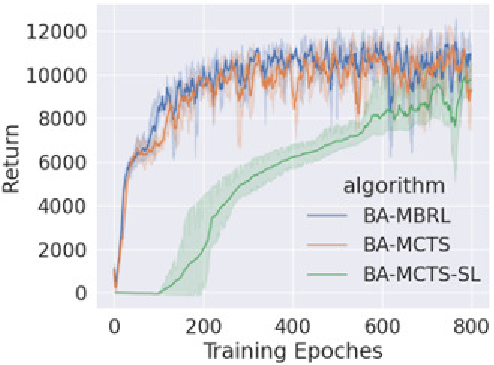
\includegraphics[width=1.5in, height=0.9in]{hc-m-exp-return-eps-converted-to.pdf}}
\subfigure[hc-med-replay]{
\label{fig:3(b)} 
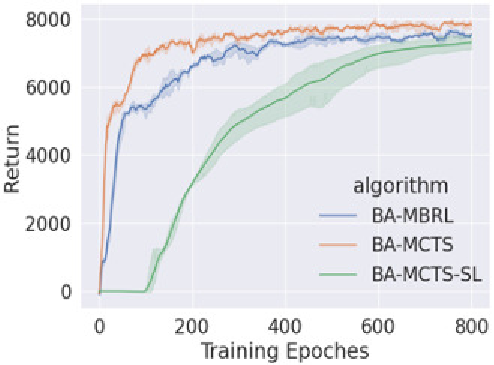
\includegraphics[width=1.5in, height=0.9in]{hc-m-rep-return-eps-converted-to.pdf}}
\subfigure[hc-medium]{
\label{fig:3(c)} 
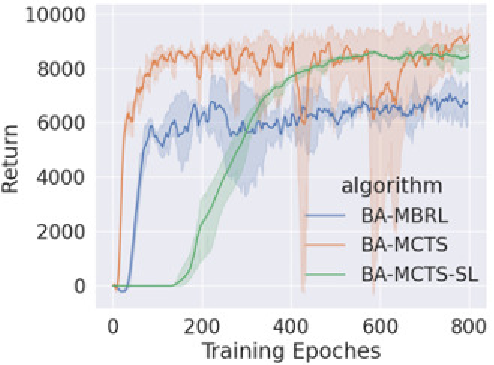
\includegraphics[width=1.5in, height=0.9in]{hc-med-return-eps-converted-to.pdf}}
\subfigure[hc-random]{
\label{fig:3(d)} 
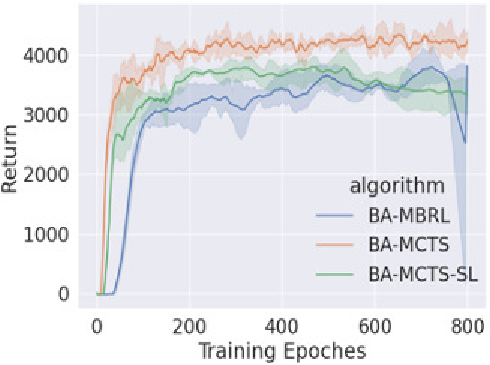
\includegraphics[width=1.5in, height=0.9in]{hc-rnd-return-eps-converted-to.pdf}}
\subfigure[hp-med-expert]{
\label{fig:3(e)} 
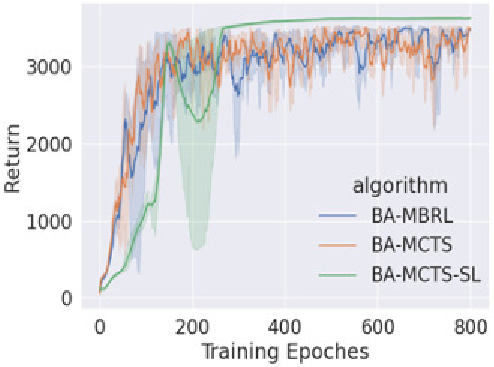
\includegraphics[width=1.5in, height=0.9in]{hp-m-exp-return-eps-converted-to.pdf}}
\subfigure[hp-med-replay]{
\label{fig:3(f)} 
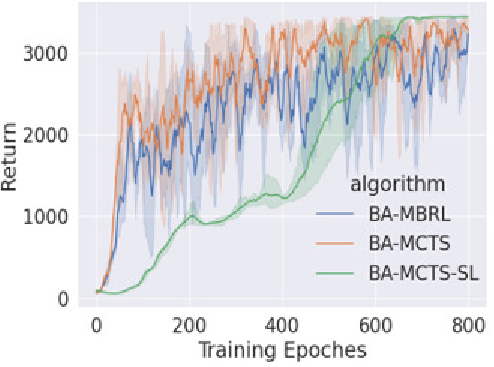
\includegraphics[width=1.5in, height=0.9in]{hp-m-rep-return-eps-converted-to.pdf}}
\subfigure[hp-medium]{
\label{fig:3(g)} 
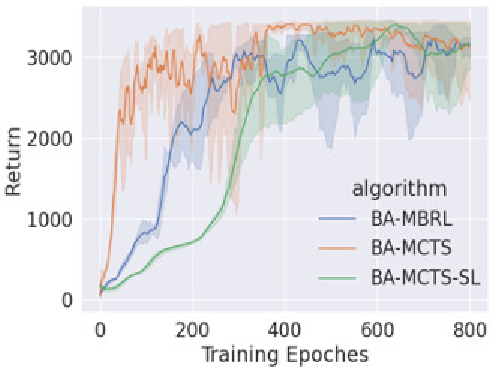
\includegraphics[width=1.5in, height=0.9in]{hp-med-return-eps-converted-to.pdf}}
\subfigure[hp-random]{
\label{fig:3(h)} 
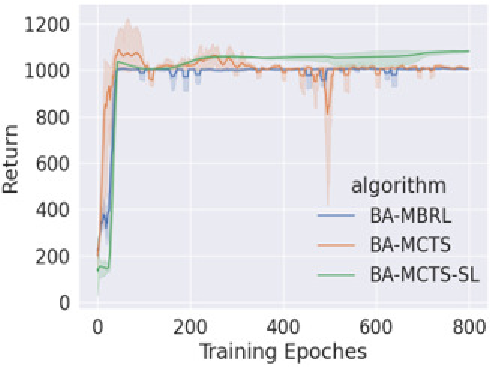
\includegraphics[width=1.5in, height=0.9in]{hp-rnd-return-eps-converted-to.pdf}}
\subfigure[wk-med-expert]{
\label{fig:3(i)} 
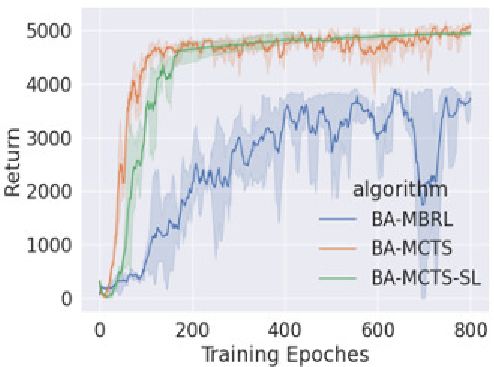
\includegraphics[width=1.5in, height=0.9in]{wk-m-exp-return-eps-converted-to.pdf}}
\subfigure[wk-med-replay]{
\label{fig:3(j)} 
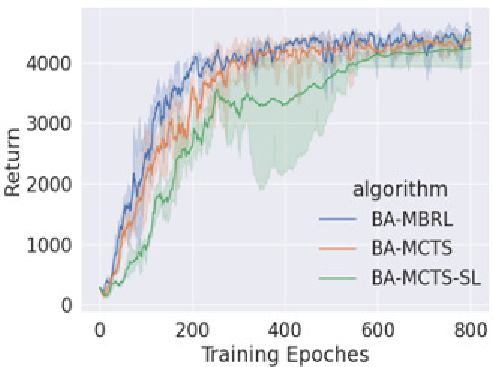
\includegraphics[width=1.5in, height=0.9in]{wk-m-rep-return-eps-converted-to.pdf}}
\subfigure[wk-medium]{
\label{fig:3(k)} 
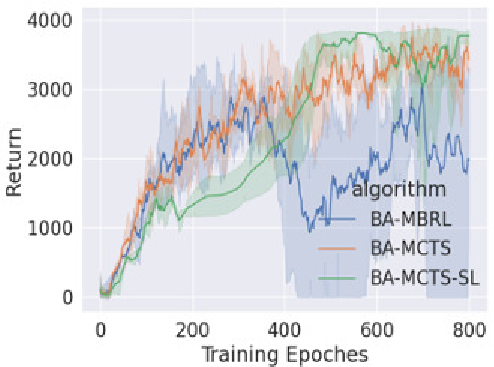
\includegraphics[width=1.5in, height=0.9in]{wk-med-return-eps-converted-to.pdf}}
\subfigure[wk-random]{
\label{fig:3(l)} 
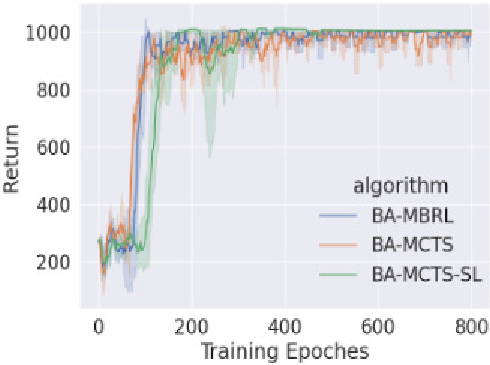
\includegraphics[width=1.5in, height=0.9in]{wk-rnd-return-eps-converted-to.pdf}}
\caption{Performance of our proposed algorithms on D4RL MuJoCo tasks. The results for HalfCheetah, Hopper, and Walker2d are presented in the three rows, respectively. Each subfigure depicts the change in the undiscounted episodic return as a function of training epochs. Experiments are repeated three times with different random seeds, with the solid line representing the mean and the shaded area indicating the 95\% confidence interval. For reference, the expert-level episodic returns for HalfCheetah, Hopper, and Walker2d are 12135, 3234.3, and 4592.3, respectively. Note that the training epochs for each algorithm, as listed in Table \ref{table:3}, have been linearly scaled to 800 for better visualization.}
\label{fig:3} 
\end{figure*}

BA-MCTS and BA-MCTS-SL utilize Bayes Adaptive Monte Carlo Tree Search to collect samples for offline model-based RL. Instead of performing a tree search at every state, we randomly select a proportion (i.e., $\rho$) of states from the available 50000 states at each rollout time step as root nodes for tree search.  For the remaining states, actions are sampled directly from the policy, i.e., $a \sim \pi(\cdot|s)$. The tree search procedure is detailed in Algorithm \ref{alg:2}, with the number of MCTS iterations, $E$, set to 50. Increasing $\rho$ and $E$ can potentially enhance performance, but it will also linearly increase the computational cost. Table \ref{table:4} outlines the key hyperparameters related to the search process for each algorithm and task. (1) As described in Algorithm \ref{alg:2}, the parameters $\alpha$ and $\beta$ control the rate of double progressive widening. ($\beta$ is set as 0.5 across all tasks.) To encourage deeper search, we limit the number of actions sampled from a state under $n_a$ and the number of next states sampled from an action under $n_s$, respectively. Action selection follows the UCT rule, as discussed in Appendix \ref{bamcp}, where $c > 0$ balances the exploration and exploitation. Additionally, inspired by the success of MuZero in enhancing exploration, we introduce Dirichlet noise $x_d$ at the root nodes, where actions are sampled from a mixture of distributions: $a \sim \eta x_d + (1-\eta) \pi(\cdot|s)$ and $\eta$ controls the mixture rate. Notably, for $(c, \eta, n_a, n_s)$, we explore the set of possible combinations: $\{(2.5, 0.3, 20, 1), (1.0, 0.3, 20, 1), (1.0, 0.1, 20, 1), (1.0, 0.3, 10, 5), (1.0, 0.1, 10, 5)\}$ during hyperparameter fine-tuning. We believe there are likely more optimal search settings yet to be discovered. (2) In BA-MCTS-SL, policy improvement is achieved through supervised learning. We find that, rather than learning solely from samples collected within the current epoch, incorporating a buffer of samples from the past $N_{SL}$ epochs helps to stabilize the learning process. Also, in the Walker2d environment, BA-MCTS-SL requires a warm-up training phase of $N_{P}$ epochs using BA-MBRL, allowing the initial policy to generate effective signals for supervised learning. 



\section{Comparisons with Model-free Methods on D4RL MuJoCo} \label{ComMF}

\begin{table}[htbp]
\scriptsize
\centering
\begin{tabular}{c|c|c|c|c|c|c|c|c|c}
\hline
{\makecell{Data Type}} & {Environment} & {\makecell{BA-MCTS \\ -SL (ours)}} & {\makecell{BA-MCTS \\ (ours)}} & {\makecell{BA-MBRL \\ (ours)}} & {CQL} & {BEAR} & {BRAC-v} & {SAC} & {BC}\\
\hline 
\hline
{random} & {HalfCheetah} & {29.20 $\pm$ 2.00} & {\textbf{36.23} $\pm$ 1.04} & {32.76 $\pm$ 1.16} & {35.4} & {25.1} & {31.2} & {30.5} & {2.1} \\
{random} & {Hopper} & {\textbf{33.83} $\pm$ 0.10} & {31.56 $\pm$ 0.12} & {31.47 $\pm$ 0.03} & {10.8} & {11.4} & {12.2} & {11.3} & {1.6} \\
{random} & {Walker2d} & {\textbf{21.89} $\pm$ 0.07} & {21.59 $\pm$ 0.32} & {21.45 $\pm$ 0.53} & {7.0} & {7.3} & {1.9} & {4.1} & {9.8}\\
\hline
{medium} & {HalfCheetah} & {70.47 $\pm$ 3.52} & {\textbf{75.84} $\pm$ 3.81} & {56.54 $\pm$ 5.20} & {44.4} & {41.7} & {46.3} & {-4.3} & {36.1}\\
{medium} & {Hopper} & {97.75 $\pm$ 7.09} & {96.70 $\pm$ 14.0} & {\textbf{98.25} $\pm$ 3.42} & {86.6} & {52.1} & {31.1} & {0.8} & {29.0}\\
{medium} & {Walker2d} & {\textbf{82.24} $\pm$ 1.85} & {74.73 $\pm$ 3.25} & {75.41 $\pm$ 4.17} & {74.5} & {59.1} & {81.1} & {0.9} & {6.6}\\
\hline 
{med-replay} & {HalfCheetah} & {61.16 $\pm$ 1.60} & {\textbf{65.45} $\pm$ 0.81} & {62.50 $\pm$ 0.18} & {46.2} & {38.6} & {47.7} & {-2.4} & {38.4}\\
{med-replay} & {Hopper} & {\textbf{106.3} $\pm$ 0.13} & {101.8 $\pm$ 3.46} & {93.91 $\pm$ 4.25} & {48.6} & {33.7} & {0.6} & {3.5} & {11.8}\\
{med-replay} & {Walker2d} & {92.13 $\pm$ 5.13} & {95.06 $\pm$ 2.11} & {\textbf{97.54}$\pm$ 1.93} & {32.6} & {19.2} & {0.9} & {1.9} & {11.3}\\
\hline 
{med-expert} & {HalfCheetah} & {80.53 $\pm$ 6.63} & {76.16 $\pm$ 10.3} & {\textbf{90.52} $\pm$ 4.13} & {62.4} & {53.4} & {41.9} & {1.8} & {35.8}\\
{med-expert} & {Hopper} & {\textbf{112.2} $\pm$ 0.29} & {108.3 $\pm$ 0.22} & {107.8 $\pm$ 0.37} & {111} & {96.3} & {0.8} & {1.6} & {111.9}\\
{med-expert} & {Walker2d} & {107.7 $\pm$ 0.82} & {\textbf{110.0} $\pm$ 1.74} & {84.71 $\pm$ 0.87} & {98.7} & {40.1} & {81.6} & {-0.1} & {6.4}\\
\hline
\hline
\multicolumn{2}{c|}{Average Score} & {\textbf{74.62}} & {74.45} & {71.06} & {54.85} & {39.83} & {31.44} & {4.13} & {25.07}\\
\hline 
\end{tabular}
\caption{Comparisons between the proposed algorithms and model-free offline policy learning methods on the D4RL benchmark suite. Each value represents the normalized score, as proposed in (\cite{DBLP:journals/corr/abs-2004-07219}), of the policy trained by the corresponding algorithm. These scores are undiscounted returns normalized to approximately range between 0 and 100, where a score of 0 corresponds to a random policy and a score of 100 corresponds to an expert-level policy. For our algorithms, we report the average score of the final ten policy learning epochs and its standard deviation across three different random seeds.}
\label{table:2}
\end{table}

As a complement to Table \ref{table:1}, we compare our algorithms with a series of model-free offline policy learning (\cite{DBLP:journals/corr/abs-2402-13777}) methods. We include SOTA model-free offline RL methods: CQL (\cite{DBLP:conf/nips/KumarZTL20}), BEAR (\cite{DBLP:conf/nips/KumarFSTL19}), and BRAC-v (\cite{DBLP:journals/corr/abs-1911-11361}). Additionally, we show the performance of directly applying SAC or Behavioral Cloning (BC, \cite{DBLP:journals/corr/abs-2402-13777}) to the provided offline dataset in the last two columns. The mean performance of the baselines are taken from related works (\cite{DBLP:conf/nips/YuTYEZLFM20, DBLP:conf/nips/KidambiRNJ20, DBLP:journals/corr/abs-2004-07219}). Our algorithms show significantly better performance, demonstrating the necessity of model-based learning in these environments. The training plots of our proposed algorithms in each environment is further detailed in Figure \ref{fig:3}.

\section{Computation Cost of Sampled EfficientZero on D4RL MuJoCo} \label{CompCost}

Here, we report the training time of Sampled EfficientZero on the D4RL MuJoCo tasks in Table \ref{table:5}. This set of experiments is run on a server with 40 Intel(R) Xeon(R) Gold 5215 CPUs and 4 Tesla V100-SXM2-32GB GPUs. Despite the substantial computational input, no corresponding performance improvement is observed. We welcome researchers to use our released code for further hyperparameter fine-tuning and to improve the results we have provided.

\begin{table}[htbp]
\centering
\begin{tabular}{c|c|c|c}
\hline
hc-med-expert & hc-med-replay & hc-medium & hc-random \\ 
\hline
55.4 $\pm$ 1.3 & 54.8 $\pm$ 1.8 & 54.7 $\pm$ 1.9 & 54.8 $\pm$ 2.6 \\
\hline
\hline
hp-med-expert & hp-med-replay & hp-medium & hp-random \\
\hline
66.1 $\pm$ 0.9 & 126.6 $\pm$ 12.0 & 70.5 $\pm$ 1.0 & 153.7 $\pm$ 19.4 \\
\hline
\hline
wk-med-expert & wk-med-replay & wk-medium & wk-random \\ 
\hline
60.8 $\pm$ 1.8 & 134.9 $\pm$ 4.2 & 63.7 $\pm$ 1.5 & 175.7 $\pm$ 28.2\\
\hline
\end{tabular}
\caption{Training time (in hours) of Sampled EfficientZero for each evaluation task. The mean and standard deviation from repeated experiments are reported.}
\label{table:5}
\end{table}

\section{Ablation Study on the Reward Penalty} \label{ASRP}

\begin{table}[htbp]
\scriptsize
\centering
\begin{tabular}{c|c|c|c|c|c|c|c}
\hline
{\makecell{Data Type}} & {Environment} & {\makecell{BA-MCTS \\ -SL}} & {\makecell{BA-MCTS}} & {\makecell{BA-MBRL}} & {\makecell{BA-MCTS \\ -SL ($\lambda=0$)}} & {\makecell{BA-MCTS \\ ($\lambda=0$)}} & {\makecell{BA-MBRL \\ ($\lambda=0$)}} \\
\hline 
\hline
{random} & {HalfCheetah} & {29.20 $\pm$ 2.00} & {36.23 $\pm$ 1.04} & {32.76 $\pm$ 1.16} & {34.80 $\pm$ 1.39} & {38.78 $\pm$ 1.65} & {\textbf{39.64} $\pm$ 2.86} \\
{random} & {Hopper} & {\textbf{33.83} $\pm$ 0.10} & {31.56 $\pm$ 0.12} & {31.47 $\pm$ 0.03} & {9.16 $\pm$ 0.16} & {7.44 $\pm$ 0.14} & {6.97 $\pm$ 0.07}\\
{random} & {Walker2d} & {\textbf{21.89} $\pm$ 0.07} & {21.59 $\pm$ 0.32} & {21.45 $\pm$ 0.53} & {17.53 $\pm$ 6.16} & {21.53 $\pm$ 0.42} & {21.41 $\pm$ 0.64}\\
\hline
{medium} & {HalfCheetah} & {70.47 $\pm$ 3.52} & {\textbf{75.84} $\pm$ 3.81} & {56.54 $\pm$ 5.20} & {61.64 $\pm$ 4.58} & {60.84 $\pm$ 2.00} & {41.49 $\pm$ 2.29}\\
{medium} & {Hopper} & {97.75 $\pm$ 7.09} & {96.70 $\pm$ 14.0} & {98.25 $\pm$ 3.42} & {102.8 $\pm$ 2.29} & {\textbf{104.4} $\pm$ 1.88} & {93.68 $\pm$ 11.4}\\
{medium} & {Walker2d} & {82.24 $\pm$ 1.85} & {74.73 $\pm$ 3.25} & {75.41 $\pm$ 4.17} & {\textbf{82.61} $\pm$ 0.86} & {57.01 $\pm$ 7.24} & {57.97 $\pm$ 15.4}\\
\hline 
{med-replay} & {HalfCheetah} & {61.16 $\pm$ 1.60} & {\textbf{65.45} $\pm$ 0.81} & {62.50 $\pm$ 0.18} & {42.10 $\pm$ 2.85} & {36.65 $\pm$ 2.39} & {44.03 $\pm$ 7.35}\\
{med-replay} & {Hopper} & {106.3 $\pm$ 0.13} & {101.8 $\pm$ 3.46} & {93.91 $\pm$ 4.25} & {\textbf{107.9} $\pm$ 0.07} & {84.11 $\pm$ 2.97} & {91.81 $\pm$ 11.5} \\
{med-replay} & {Walker2d} & {92.13 $\pm$ 5.13} & {95.06 $\pm$ 2.11} & {97.54$\pm$ 1.93} & {88.61 $\pm$ 5.21} & {97.33 $\pm$ 3.51} & {\textbf{98.19} $\pm$ 1.23}\\
\hline 
{med-expert} & {HalfCheetah} & {80.53 $\pm$ 6.63} & {76.16 $\pm$ 10.3} & {\textbf{90.52} $\pm$ 4.13} & {51.76 $\pm$ 5.31} & {26.60 $\pm$ 1.46} & {29.88 $\pm$ 2.28}\\
{med-expert} & {Hopper} & {\textbf{112.2} $\pm$ 0.29} & {108.3 $\pm$ 0.22} & {107.8 $\pm$ 0.37} & {106.8 $\pm$ 6.34} & {81.76 $\pm$ 6.45} & {86.79 $\pm$ 18.7}\\
{med-expert} & {Walker2d} & {107.7 $\pm$ 0.82} & {110.0 $\pm$ 1.74} & {84.71 $\pm$ 0.87} & {\textbf{110.8} $\pm$ 1.72} & {110.2 $\pm$ 0.91} & {53.35 $\pm$ 38.0}\\
\hline
\hline
\multicolumn{2}{c|}{Average Score} & {\textbf{74.62}} & {74.45} & {71.06} & {68.04} & {60.55} & {55.43} \\
\hline 
\end{tabular}
\caption{Comparison of the proposed algorithms with their corresponding versions without the reward penalty (i.e., $\lambda=0$). The definitions of the values in this table are consistent with those in Table \ref{table:2}.}
\label{table:8}
\end{table}

To demonstrate the necessity of incorporating the reward penalty in offline MBRL, we conduct an ablation study by setting $\lambda$ in Eq. (\ref{p-rwd}) to 0, resulting in ablated versions of our proposed three algorithms. The results are presented in Table \ref{table:8}. \textbf{First}, the average performance of the algorithms with the reward penalty is consistently better, demonstrating the importance of using reward penalties in offline MBRL to prevent the overexploitation of the learned world models (which can be inaccurate). \textbf{Second}, the supervised-learning-based algorithm (i.e., BA-MCTS-SL ($\lambda=0$)) is less affected by the absence of the reward penalty, compared to the policy-gradient-based methods. Notably, BA-MCTS-SL ($\lambda=0$) and BA-MCTS-SL achieve comparable performance in the Hopper and Walker2d tasks. This shows an additional advantage of BA-MCTS-SL -- its reduced sensitivity to model inaccuracies. \textbf{Lastly}, there are instances where superior performance is achieved with $\lambda$ set to 0. For example, BA-MCTS-SL ($\lambda=0$) performs better than BA-MCTS-SL in 5 out of 12 tasks. This suggests that the performance of our algorithms in Tables \ref{table:1} and \ref{table:2} could be further improved by adjusting hyperparameters such as $\lambda$\footnote{As mentioned in Section \ref{eval}, we retain most of the hyperparameter settings from Optimized (\cite{DBLP:conf/iclr/LuBPOR22}) to ensure that the performance improvements are attributed to our algorithm design.}.

\section{Details of the Tokamak Control Tasks} \label{DetTCT}

\begin{table}[htbp]
\small
\centering
\begin{tabular}{|c||c|}
\hline
\multicolumn{2}{|c|}{STATE SPACE} \\
\hline
{Scalar States} & \makecell{$\beta_n$, Internal Inductance, Line Averaged Density,\\ Loop Voltage, Stored Energy} \\
\hline
{Profile States} & \makecell{Electron Density, Electron Temperature, Pressure,\\ Safety Factor, Ion Temperature, Ion Rotation} \\
\hline
\multicolumn{2}{c}{}\\[-0.5em]
\hline
\multicolumn{2}{|c|}{ACTION SPACE} \\
\hline
{Targets} & {Current Target, Density Target} \\
\hline
{Shape Variables} & \makecell{Elongation, Top Triangularity, Bottom Triangularity, Minor Radius, \\Radius and Vertical Locations of the Plasma Center} \\
\hline
{Direct Actuators} & \makecell{Power Injected, Torque Injected, Total Deuterium Gas Injection,\\ Total ECH Power, Magnitude and Sign of the Toroidal Magnetic Field} \\
\hline
\end{tabular}
\caption{The state and action spaces of the tokamak control tasks.}
\label{table:7}
\end{table}

Nuclear fusion is a promising energy source to meet the world’s growing demand. It involves fusing the nuclei of two light atoms, such as hydrogen, to form a heavier nucleus, typically helium, releasing energy in the process. The primary challenge of fusion is confining a plasma, i.e., an ionized gas of hydrogen isotopes, while heating it and increasing its pressure to initiate and sustain fusion reactions. The tokamak is one of the most promising confinement devices. It uses magnetic fields acting on hydrogen atoms that have been ionized (given a charge) so that the magnetic fields can exert a force on the moving particles (\cite{1512794}). 

\cite{DBLP:journals/corr/abs-2404-12416} trained a deep recurrent network as a dynamics model for the DIII-D tokamak, a device located in San Diego, California, and operated by General Atomics, using a large dataset of operational data from that device. A typical shot (i.e., episode) on DIII-D lasts around 6-8 seconds, consisting of a one-second ramp-up phase, a multi-second flat-top phase, and a one-second ramp-down phase. The DIII-D also features several real-time and post-shot diagnostics that measure the magnetic equilibrium and plasma parameters with high temporal resolution. The authors demonstrate that the learned model predicts these measurements for entire shots with remarkable accuracy. Thus, we use this model as a ``ground truth" simulator for tokamak control tasks. Specifically, we generate a dataset of 725270 transitions for offline RL and evaluate the learned policy using this data-driven simulator.

The state and action spaces for the tokamak control tasks are outlined in Table \ref{table:7}. For detailed physical explanations of their components, please refer to (\cite{abbate2021data, DBLP:conf/l4dc/CharABBCCEMRKS23, ariola2008magnetic}). The state space consists of five scalar values and six profiles which are discretized measurements of physical quantities along the minor radius of the toroid. After applying principal component analysis (\cite{mackiewicz1993principal}), the pressure profile is reduced to two dimensions, while the other profiles are reduced to four dimensions each. In total, the state space comprises 27 dimensions. The action space includes direct control actuators for neutral beam power, torque, gas, ECH power, current, and magnetic field, as well as target values for plasma density and plasma shape, which are managed through a lower-level control module. Altogether, the action space consists of 14 dimensions. While for certain tasks, it is possible to prune the state and action spaces to reduce the learning complexity, we have chosen not to apply any domain-specific knowledge in these evaluations for general RL algorithms. We reserve the domain-specific applications of our algorithms, which would require more domain knowledge and engineering efforts, as an important future work.

We select a reference shot from DIII-D, which spans 251 time steps, and use its trajectories of Ion Rotation, Electron Temperature, and $\beta_n$ as targets for three tracking tasks. Specifically, $\beta_n$ is the normalized ratio between plasma pressure and magnetic pressure, a key quantity serving as a rough economic indicator of efficiency. Since the tracking targets vary over time, we include the time step as part of the policy input. The reward function for each task is defined as the negative squared tracking error of the corresponding component (i.e., temperature, rotation, or $\beta_n$) at each time step, and the reward is normalized by the episode horizon (i.e., 251 time steps). Notably, for policy learning, the reward function is provided rather than learned from the offline dataset as in D4RL tasks; and the dataset does not include the reference shot or any nearby, similar shots.







